\documentclass[9pt]{beamer}

\mode<presentation> {\usetheme{Kaiping}}

\usepackage[ngerman]{babel}

\usepackage{fontspec}
\setmainfont{Linux Biolinum}
%\setmonofont{Linux Biolinum}
\setsansfont{Linux Biolinum}

\usepackage{xcolor}
\usepackage{graphicx}
\usepackage{tikz}
\usepackage{tikz-cd}

\usefonttheme[onlymath]{serif}
\usetheme{Warsaw}
% default
% Boadilla
% Madrid
% Pittsburgh
% Rochester \usetheme[height=7mm]{Rochester}
% Copenhagen
% Warsaw
% Singapore
% Malmoe

% Decrease footnote size

\title{Growing Trees from Big Data}
\subtitle{Bayesian Phyologeny for Historical Linguistics}
\author{Gereon Kaiping}
%\institute{Leiden University Centre for Linguistics, the Netherlands}
\date{20-3-2017}

\begin{document}

\begin{frame}[plain]
  \titlepage
\end{frame}
\begin{frame}
  \tableofcontents
\end{frame}
\section{Solutions to All Your Problems!}
\subsection{Crunching Numbers}
\begin{frame}{Problem}
  Using the comparative method is hard, because
  \begin{itemize}
  \item it is a lot of painstaking work,
  \item we don't know how to weigh the evidence,
  \item cognates may have changed meanings,
  \item loan words make our lives more difficult.
  \end{itemize}
  And then doesn't even give us dates, just “not before” or “not after” if we are lucky.
\end{frame}
\begin{frame}{Solution}
  \textbf{Bayesian Phylogenetic Inference}, from biology
  
  \textit{Idea:} Evolution = a random process on a tree. What tree is most probable?
  \begin{tikzpicture}
    \node<1->[align=left,anchor=east] (arrow) at (0,0) {→};
    \node<1>[align=left,anchor=east,font={\scshape\ttfamily}] at (arrow.west) {
      cctccacgcc aacggagcct cattcttctt\\
      cctccacgcc aacaaagcct cattctt---\\
      cctccacgcc aacaaagcct cattcttctt\\
      cctccacgcc aacggagcct caggtgtctt\\
      cctccactcc aacggagcct caggtgtctt};
    \node<2->[align=left,anchor=east,red,font={\scshape\ttfamily}] at (arrow.west) {
      cctccacgcc some agcct cattcttctt\\
      cctccacgcc language t cattcttctt\\
      cctccacgcc data agcct cattcttctt\\
      cctccacgcc aacggagcct cattcttctt\\
      cctccactcc aacggagcct caggtgtctt};
    \node<1->[anchor=west,inner sep=0] (image) at (0,0) {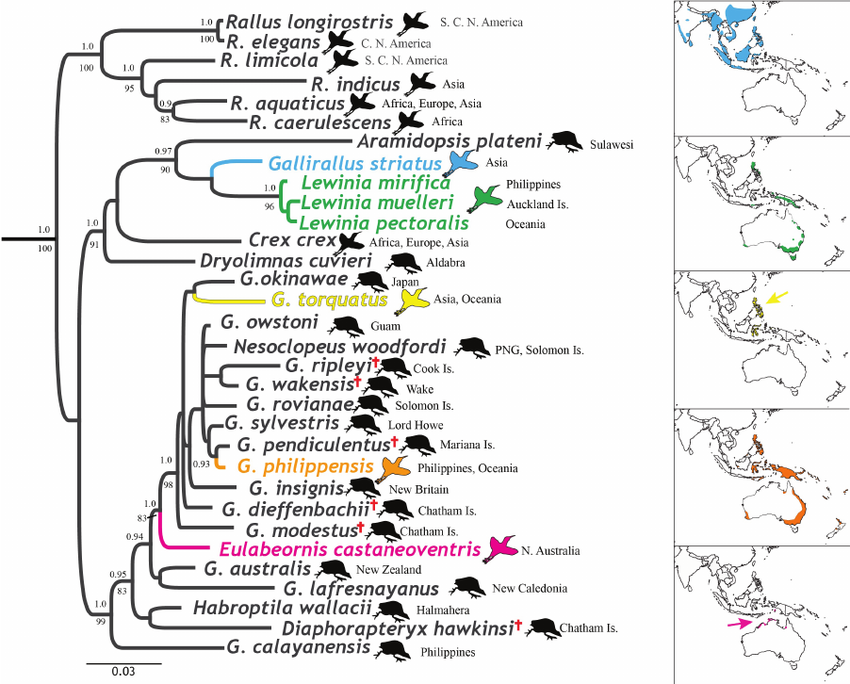
\includegraphics[width=0.5\textwidth,trim={0 0 7cm 0},clip]{Bayesian-Rallus.png}};
    \node<2->[align=right,red,font={\Huge\bfseries}] at (image.center) {Flemish\\Dutch\\German\\Frisian\\English\\Swedish\\Danish\\Norwegian};
  \end{tikzpicture}
\end{frame}
\subsection{Bayesian …}
\begin{frame}{Bayes' Theorem}
  Probabilities = confidence of belief, not random experiment.
  “What are consistent beliefs?”
  \begin{align}
    P(\text{Model} \mid \text{Data}) \propto P(\text{Data} \mid \text{Model}) \times P(\text{Model})
  \end{align}
  \begin{center}
    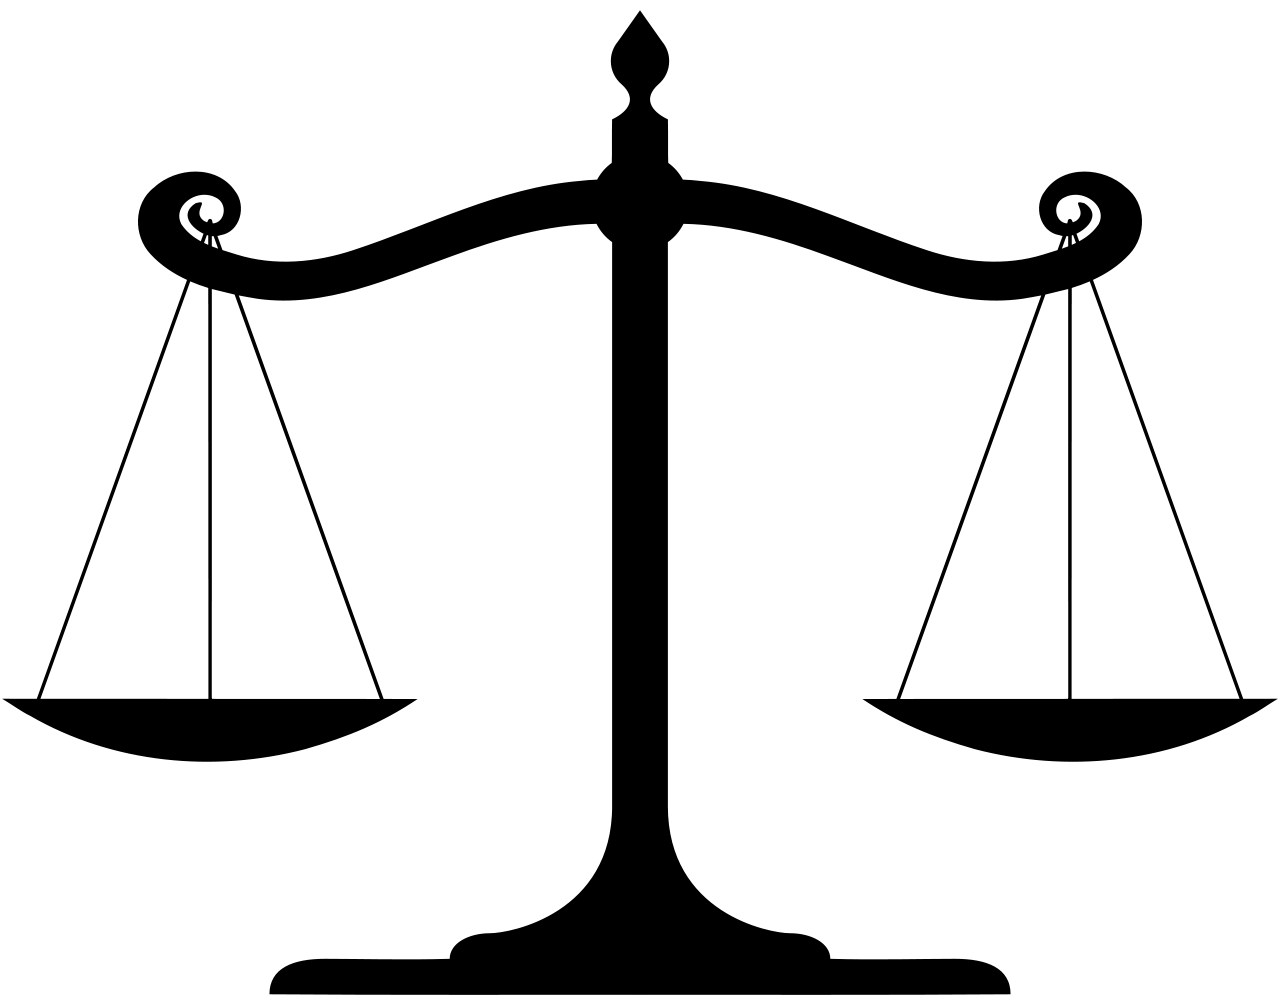
\includegraphics[width=0.3\textwidth]{scale.png}
  \end{center}
\end{frame}
\subsection{… Phylogenetics}
\begin{frame}{Computational Phylogenetics}
\end{frame}
\section{[Examples]}
\subsection{Austronesian: Branches and times}
\begin{frame}{Example 1: Austronesian}
  \begin{columns}
    \begin{column}{0.5\textwidth}
      \includegraphics[width=\textwidth,page=2,trim={2cm 4cm 1cm 5cm},clip]{austronesian.pdf}
    \end{column}
    \begin{column}{0.5\textwidth}
      \footnotesize “The invention of the outrigger canoe and its
        sail may have enabled the Austronesians to move across this
        channel before spreading rapidly over the 7000 km from the
        Philippines to Polynesia (4). This is supported by linguistic
        reconstructions showing that the terminology associated with
        the outrigger canoe complex can only be traced back to Proto-
        Malayo-Polynesian and not Proto-Austronesian (41).”
      \includegraphics[width=0.6\textwidth,page=3,trim={1cm 1cm 7.5cm 16cm},clip]{austronesian.pdf}
    \end{column}
  \end{columns}
\end{frame}
\subsection{Bantu: Phylogeography}
\begin{frame}{Example 2: Bantu}
  \begin{columns}
    \begin{column}{0.5\textwidth}
      \includegraphics[width=\textwidth,page=5,trim={5cm 11.5cm 3cm 1cm},clip]{bantu.pdf}
    \end{column}
    \begin{column}{0.5\textwidth}
      \footnotesize “[…] explicit mapping of ancestral locations to make
      inferences about the specific route taken during the dispersal
      of Bantu languages. The results clearly support the ‘pathway
      through the rainforest’ scenario for the expansion of Bantu
      through much of sub-Saharan Africa. There is no support
      in these analyses for an early, deep split between East and
      West Bantu languages and a movement by one branch
      north of the rainforest.”
    \end{column}
  \end{columns}
\end{frame}
\section{And why actually not.}
\begin{frame}{Criticism}
  \begin{itemize}
  \item Model realism
  \item Disregarding prior knowledge
  \item Data vetting
  \end{itemize}
\end{frame}
\section{Conclusions}
\begin{frame}{Conclusions}
  \begin{itemize}
  \item Computer models can help make sense of large data sets
  \item Mathematical models can handle new \emph{types} of data for new types of results
  \item Very few language-specific models so far
  \item If you disagree with results, \emph{what parameters or choices do you disagree with?}
  \end{itemize}
\end{frame}
\subsection{Further Reading}
\begin{frame}
  Course
  Literature: McMahon \& McMahon
\end{frame}
\end{document}
%%% Local Variables:
%%% TeX-engine: luatex
%%% End: 
